\chapter{Caja protectora del sistema}

\section*{Resumen}
Este capítulo detalla el diseño mecánico y la fabricación mediante impresión 3D del encapsulado del sistema de radar. El encapsulado garantiza la protección física de los circuitos y la seguridad del operador durante la toma de mediciones y el transporte, manteniendo accesibles únicamente los puertos de conexión estrictamente necesarios.

\section{Introducción}
La viabilidad operativa de un instrumento de medición requiere, además de un correcto diseño electrónico, de una estructura física que garantice su integridad. El desarrollo de un encapsulado a medida resulta fundamental para aislar los módulos sensibles, prevenir cortocircuitos por contacto accidental y facilitar el transporte del equipo en entornos de prueba. En este capítulo se presenta el proceso de modelado tridimensional y la posterior materialización del chasis protector del radar.

\section{Desarrollo de la caja protectora}
Como parte de la implementación final del radar se desarrolló un encapsulado destinado a proteger los circuitos y componentes que conforman el sistema. Además de proporcionar protección mecánica durante el transporte y la realización de mediciones, la caja permite evitar el contacto accidental con puntos de alimentación, conexiones y componentes que no deben ser manipulados durante el funcionamiento del equipo.

El encapsulado fue diseñado en Onshape, como se observa en la Figura~\ref{fig:encapsulado_radar1}, considerando la disposición de los diferentes módulos del radar y permitiendo mantener accesibles únicamente las conexiones necesarias para su operación.

\begin{figure}[H]
\centering
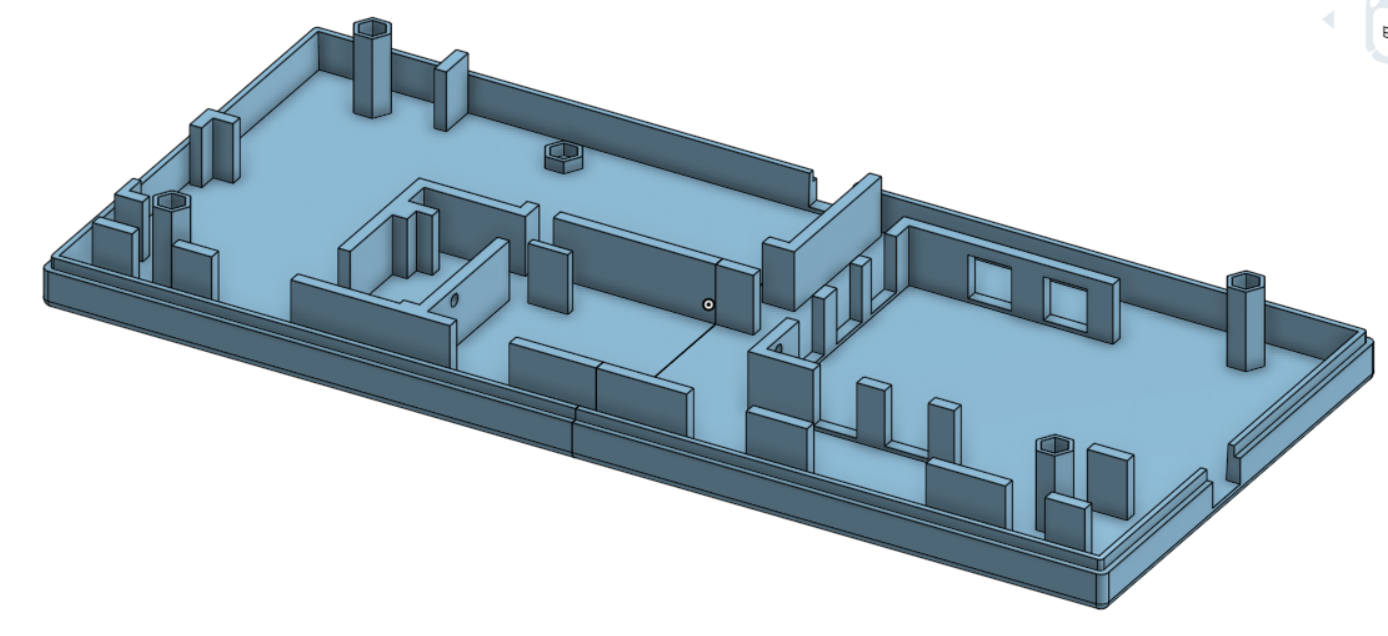
\includegraphics[width=0.65\textwidth]{imagenes/encapsulado_radar.png}
\caption{Diseño CAD del encapsulado del sistema de radar en Onshape. (Fuente: Propia).}
\label{fig:encapsulado_radar1}
\end{figure}

Posteriormente fue fabricado mediante una impresora 3D, obteniendo el resultado que se muestra en la Figura~\ref{fig:encapsulado_radar}.

\begin{figure}[H]
    \centering
    \begin{subfigure}[b]{0.6\textwidth}
        \centering
        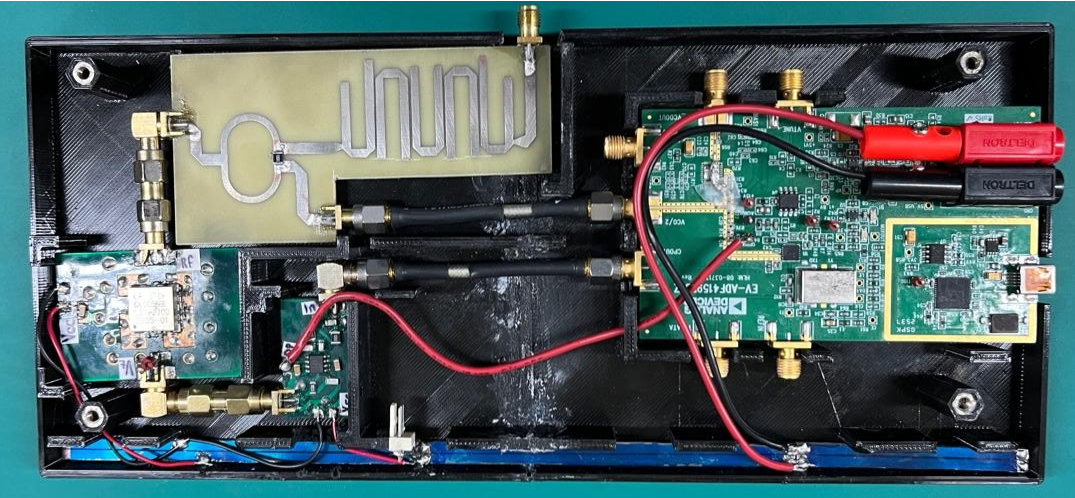
\includegraphics[width=\textwidth]{imagenes/sistemacaja1.png}
        \caption{Caja abierta con los módulos integrados.}
        \label{fig:caja_abierta}
    \end{subfigure}

    \vspace{0.3cm}

    \begin{subfigure}[b]{0.6\textwidth}
        \centering
        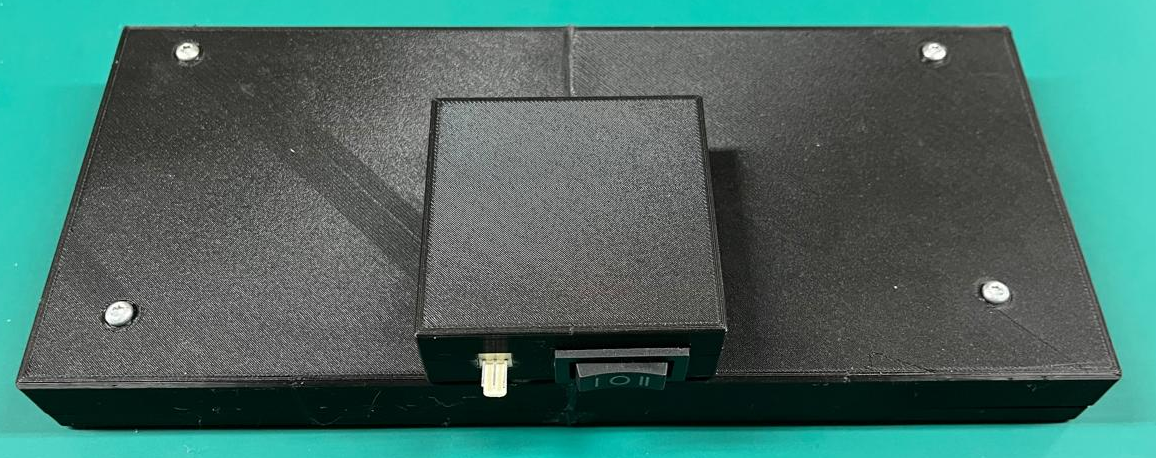
\includegraphics[width=\textwidth]{imagenes/sistemacaja2.png}
        \caption{Caja cerrada.}
        \label{fig:caja_cerrada}
    \end{subfigure}

    \caption{Encapsulado del sistema de radar fabricado en impresión 3D. (Fuente: Propia).}
    \label{fig:encapsulado_radar}
\end{figure}